\documentclass[12pt,a4paper]{article}
\usepackage{fontspec, xunicode, xltxtra}
\XeTeXlinebreaklocale "zh"
\XeTeXlinebreakskip = 0.1pt plus 1pt minus 0.1pt
\usepackage{xeCJK} 
\usepackage{fontspec}  
\setCJKmainfont{SimSun} 
\setCJKmonofont{SimSun} 
\setmainfont{Courier}%{Times New Roman} {SourceCodePro-Regular}{Consolas}{Courier}
\usepackage{indentfirst} 
\setlength{\parindent}{2em}
\usepackage{float}
\usepackage[utf8]{inputenc}
\usepackage{setspace}
\usepackage[colorlinks,linkcolor=black,anchorcolor=black,citecolor=black]{hyperref}
\usepackage{amsmath}
\usepackage{amsfonts}
\usepackage{amssymb}
\usepackage{geometry}
\geometry{left=2.5cm,right=2.5cm,top=2.5cm,bottom=4cm}
\usepackage{listings}
\lstset{language=C++}
\lstset{breaklines}
\lstset{extendedchars=false}
\usepackage{fancyhdr}
\pagestyle{fancy}
\lhead{数据结构大作业报告}
\author{姚皓天(2013011515)}
\title{数据结构大作业报告\\八数码}
\date{2014年11月}

\begin{document}
\maketitle
\thispagestyle{empty}

\newpage
\thispagestyle{empty}
\renewcommand\contentsname{\textbf{目录}}
\tableofcontents

\newpage
\section{基本原理}
\subsection{概述}
本程序采用Microsoft Visual Studio 2012 的“MFC应用程序”开发,实现了简单地八数码的搜索算法和演示功能。实现了三种算法,深搜、广搜、和A*算法。

因为程序功能有限,使用了基本的单对话框模板实现程序功能。
\subsection{原理}
在MFC的基本框架之上,首先编写了EightFigureState类,用于统一使用一个int变量来描述八数码的的状态,同时还保存搜索中产生的相关信息。SearchCore类作为作为基类派生所有的搜索方法。CEightFigureDlg类用于控制图形界面。
\subsection{特色}
\begin{itemize}
\item 使用SearchCore类作为作为基类,派生出所有的搜索方法,每个方法复写虚函数Search,使用统一的接口,方便编程与扩展。
\item 开发过程中使用了VS的单元测试框架对几个重要类的方法进行了测试,大大提高了开发成功率,缩短了开发时间。
\item 搜索中访问过的状态使用Hash Set保存,可以取得很快的速度。
\end{itemize}
\subsection{界面}
\begin{figure}[H]
\centering
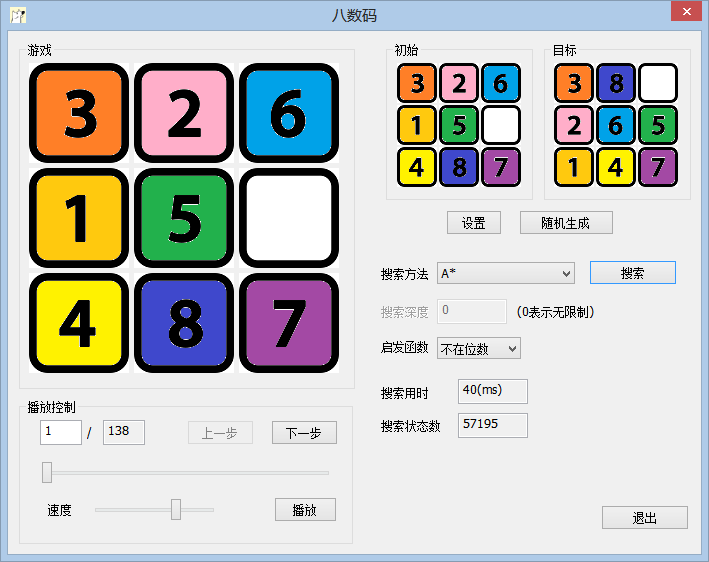
\includegraphics[width=0.8\textwidth]{1.png}
\caption{界面} 
\end{figure}
\subsection{操作说明}
\subsubsection{始末状态}
始末状态可以手动设置,也可以随机生成。(始末状态会通过逆序数方法检查是否可解,如果不可解就会提示用户;随机生成的组合都是可解的)
\subsubsection{搜索方法}
程序提供了3种搜索方法,可以通过下拉列表选择。
\subsubsection{结果演示}
结果会在左侧显示,操作方法与普通视频播放器的风格类似,右侧给出了搜索用时和访问的状态数。
\section{程序设计}
\subsection{需求分析}
程序需要采用不同的搜索方法来求解八数码问题。
\subsection{概要设计}
在MFC的基本框架之上,首先编写了EightFigureState类,用于统一使用一个int变量来描述八数码的的状态,同时还保存搜索中产生的相关信息。SearchCore类作为作为基类派生所有的搜索方法。CEightFigureDlg类用于控制图形界面。
\subsection{详细设计}
\subsubsection{EightFigureState类}
EightFigureState类,用于统一使用一个int变量来描述八数码的的状态,同时还保存搜索中产生的相关信息,并配合封装了一些方法来实现基本的功能。
\begin{lstlisting}
class EightFigureState
{
private:
   	.....
public:
    int data;			//使用一个int类型表示八数码的状态
    int depth;
    int selfIdx;
    int fatherIdx;		//搜索过程中父节点的编号
    int fVaule;			//启发函数计算值
    ......
    bool Move(Direction direction);		
    	//控制空白块向某个方向移动
    bool CanSolve(EightFigureState c);
    bool operator == (EightFigureState c);
    void operator = (EightFigureState c);
};
\end{lstlisting}
\subsubsection{SearchCore类}
SearchCore类作为所有搜索方法的基类,用于规定统一的接口
\begin{lstlisting}
class SearchCore
{
public:
    void SetStart(EightFigureState state);
    void SetTarget(EightFigureState state);
    void GetPath(std::vector<EightFigureState> &path);
    int GetTime();
    int GetStateCount();
    virtual bool Search() = 0;			
    	//定义了虚函数,在子类中实现搜索方法
protected:
    EightFigureState startState;
    EightFigureState targetState;
    std::vector<EightFigureState> path;		
   		 //vector 保存搜索出的路径
    std::hash_set<unsigned int> close;			
    	//hash set 用于保存访问过的状态
    clock_t startTime;									
   		 //记录算法运行时间
    clock_t stopTime;
};
\end{lstlisting}
\subsubsection{搜索方法}

\section{设计心得}
\subsection{收获}
感觉在这次程序设计中类的编写和封装比上一次的实现有了提高,整个编程思路变清晰了。\par
而且在这次开发中使用了VS的单元测试框架,进行了一些单元测试,提高了开发的成功率,减少了调试消耗的时间,单元测试是一种很好的方法,以后会一直使用。
\begin{figure}[H]
\centering
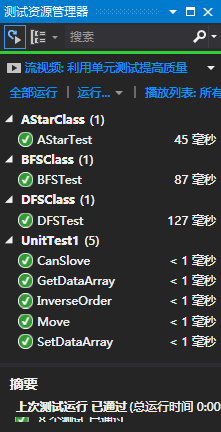
\includegraphics{2.png}
\caption{单元测试} 
\end{figure}
\subsection{问题}
A*算法中,估值函数的选取是一个值得分析的问题。
\section{文件清单}
\begin{itemize}
\item src$\backslash$ 工程文件
\begin{itemize}
\item src$\backslash$ EightFigure $\backslash$
\begin{itemize}
\item EightFigureState.h/.cpp EightFigureState类——用于描述八数码的状态
\item SearchCore.h/.cpp SearchCore类——所有搜索方法的基类
\item DFS.h/.cpp ——深搜算法
\item BFS.h/.cpp ——广搜算法
\item AStar.h/.cpp ——A*算法
\item EightFigureDlg.h/.cpp  界面对话框控制
\end{itemize}
\item src$\backslash$ UnitTest $\backslash$ 单元测试
\end{itemize}

\item bin$\backslash$ 可执行文件
\item doc$\backslash$ 文档
\end{itemize}
程序版本库:\url{https://github.com/yht1995/EightFigure.git}
\end{document}